% Options for packages loaded elsewhere
\PassOptionsToPackage{unicode}{hyperref}
\PassOptionsToPackage{hyphens}{url}
%
\documentclass[
]{article}
\title{Credit Easing, ETF Flows and Transfer Entropy}
\author{Lisha Li \and Barry Quinn \and Lisa Sheenan}
\date{2022-03-09}

\usepackage{amsmath,amssymb}
\usepackage{lmodern}
\usepackage{iftex}
\ifPDFTeX
  \usepackage[T1]{fontenc}
  \usepackage[utf8]{inputenc}
  \usepackage{textcomp} % provide euro and other symbols
\else % if luatex or xetex
  \usepackage{unicode-math}
  \defaultfontfeatures{Scale=MatchLowercase}
  \defaultfontfeatures[\rmfamily]{Ligatures=TeX,Scale=1}
\fi
% Use upquote if available, for straight quotes in verbatim environments
\IfFileExists{upquote.sty}{\usepackage{upquote}}{}
\IfFileExists{microtype.sty}{% use microtype if available
  \usepackage[]{microtype}
  \UseMicrotypeSet[protrusion]{basicmath} % disable protrusion for tt fonts
}{}
\makeatletter
\@ifundefined{KOMAClassName}{% if non-KOMA class
  \IfFileExists{parskip.sty}{%
    \usepackage{parskip}
  }{% else
    \setlength{\parindent}{0pt}
    \setlength{\parskip}{6pt plus 2pt minus 1pt}}
}{% if KOMA class
  \KOMAoptions{parskip=half}}
\makeatother
\usepackage{xcolor}
\IfFileExists{xurl.sty}{\usepackage{xurl}}{} % add URL line breaks if available
\IfFileExists{bookmark.sty}{\usepackage{bookmark}}{\usepackage{hyperref}}
\hypersetup{
  pdftitle={Credit Easing, ETF Flows and Transfer Entropy},
  pdfauthor={Lisha Li; Barry Quinn; Lisa Sheenan},
  hidelinks,
  pdfcreator={LaTeX via pandoc}}
\urlstyle{same} % disable monospaced font for URLs
\usepackage[margin=1in]{geometry}
\usepackage{graphicx}
\makeatletter
\def\maxwidth{\ifdim\Gin@nat@width>\linewidth\linewidth\else\Gin@nat@width\fi}
\def\maxheight{\ifdim\Gin@nat@height>\textheight\textheight\else\Gin@nat@height\fi}
\makeatother
% Scale images if necessary, so that they will not overflow the page
% margins by default, and it is still possible to overwrite the defaults
% using explicit options in \includegraphics[width, height, ...]{}
\setkeys{Gin}{width=\maxwidth,height=\maxheight,keepaspectratio}
% Set default figure placement to htbp
\makeatletter
\def\fps@figure{htbp}
\makeatother
\setlength{\emergencystretch}{3em} % prevent overfull lines
\providecommand{\tightlist}{%
  \setlength{\itemsep}{0pt}\setlength{\parskip}{0pt}}
\setcounter{secnumdepth}{-\maxdimen} % remove section numbering
\ifLuaTeX
  \usepackage{selnolig}  % disable illegal ligatures
\fi

\begin{document}
\maketitle

\hypertarget{introduction}{%
\section{Introduction}\label{introduction}}

Quantitative easing (QE), basically the expansion of a central bank's
balance sheet by means of the large scale purchase of government bonds
or other assets with the aim of stimulating the economy,originated in
Japan in 2001. QE focuses on bank reserves, or central bank liabilities.
The term credit easing (CE) was coined in 2009 by Ben Bernanke, the then
Chairman of the Federal Reserve,and focuses on the asset side of the
balance sheet with the aim of stimulating credit markets.These markets
were hit hard during the global financial crisis of 2007-2008 and
central banks like the Federal Reserve and the ECB began introducing
credit support measures in its aftermath in an effort to aid recovery
and trigger growth. These are part of a suite of unconventional monetary
policy measures implemented by central banks in recent years.

On 31st January 2020 the World Health Organisation (WHO) declared a
global health emergency due to the COVID-19 pandemic, leading to
lockdowns across the globe and, with this, a slowdown in the global
economy and need for large scale assistance measures. On 23rd March 2020
the Federal Reserve announced the establishment of the Primary Market
Corporate Credit Facility(PMCCF) and the Secondary Corporate Credit
Facility (SMCCF), both aimed at supporting corporate bond markets. The
SMCCF involves the purchase of corporate bonds in the secondary market,
as well as U.S.-listed exchange-traded funds (ETFs).The European Central
Bank had introduced a similar credit support program in June 2016 with
the Corporate Sector Purchase Program (CSPP), which was then expanded on
18th March 2020 to include non-financial commercial paper, thus making
all qualifying commercial papers eligible for purchase under the
program.Although ETFs are not eligible for purchase under the CSPP
following the initial announcement(and prior to the release of full
details) of the program on 10th March 2016 corporate bond ETF trading
boomed. The website ETFStrategy.com reported

\begin{quote}
Data from European-listed ETF trading platform Tradeweb showed that
trading in fixed income ETFs increased to 50.3\% as a proportion of
overall traded volume. The majority of this, 62.9\%, was in corporate
and high yield bonds, with `buys' in corporate bond ETFs nearly double
the amount of `sells'.
\end{quote}

We investigate the dynamic impact of fixed income ETF fund flows and
central bank interest rates. Specifically, we assume that there is a
substantive non-linear dynamic structure to bivariate relationships. We
assess the bivariate information flow between fixed income ETFs and
LIBOR interest rates using transfer entropy, a model-free measure of the
asymmetric information flow between time series in a network. This is a
popular approach to information diffusion and contagion in a complex
systems such as global capital markets{[}@Bekiros2017,@Nam2019{]}.

\hypertarget{data}{%
\section{Data}\label{data}}

The data is sourced from Bloomberg and consists of daily indices
capturing net ETF Flows into different bond categories of ETF in the US
market. The data is for the period 2020-03-02 - 2021-08-27. The sample
also include three interest ratios, US 3-month LIBOR, EU 3-Month LIBOR
and the SONIA interest rate benchmark.

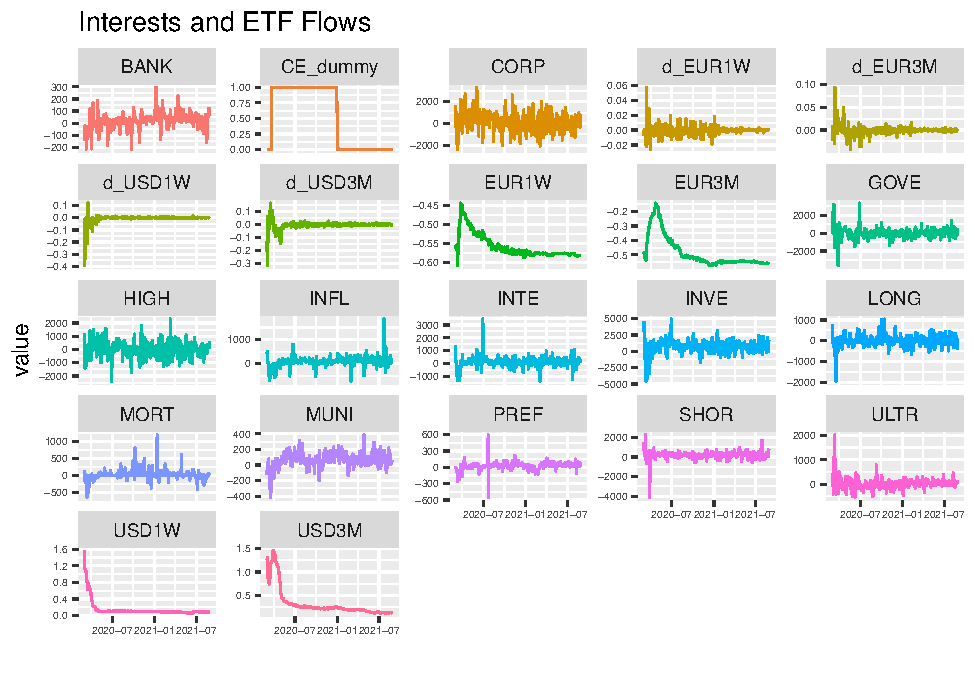
\includegraphics{working_paper_files/figure-latex/plot-1.pdf}

\hypertarget{linear-pairwise-correlations}{%
\subsection{Linear pairwise
correlations}\label{linear-pairwise-correlations}}

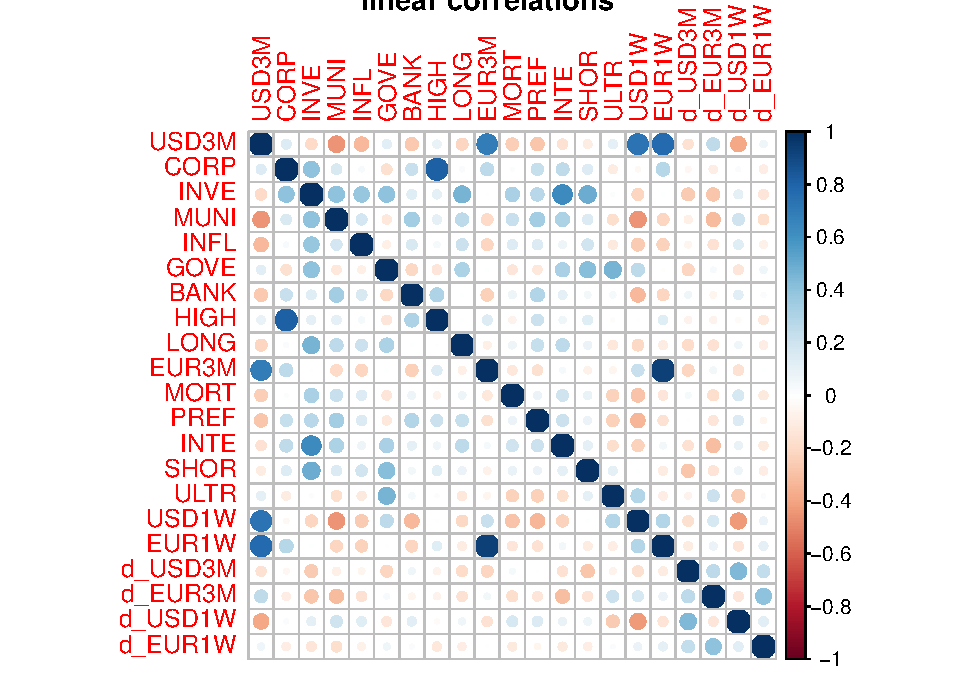
\includegraphics{working_paper_files/figure-latex/correlation-1.pdf}
Some obvious correlation in the three interest rates. There are also
some strong correlations among the ETF bond flows that will require
careful consideration. Is this due to overlapping categorisation?

\hypertarget{information-transfer-measurement}{%
\subsection{Information transfer
measurement}\label{information-transfer-measurement}}

The quantification of information transfer commonly relies on measures
that have been derived from subject-specific assumptions and
restrictions concerning the underlying stochastic processes or
theoretical models. With the development of transfer entropy,
information theory based measures have become a popular alternative to
quantify information flows within various disciplines. Transfer entropy
is a non-parametric measure of directed, asymmetric information transfer
between two processes. We quantify the information flow between two
stationary time series and test for its statistical significance using
Shannon transfer entropy(TE)\footnote{We use the package
  \texttt{RTransferEntropy}}.

In the literature, the Granger causality has been addressed in many
fields, including finance. Despite its success in the identification of
couplings between the interacting variables, the use of structural
models restricts its performance. Unlike Granger causality, TE is a
quantity that is directly estimated from data and it does not suffer
from such constraints. In the specific case of Gaussian distributed
random variables, equivalence between TE and Granger causality has been
proven.

\hypertarget{measuring-information-flows-using-transfer-entropy}{%
\subsection{Measuring information flows using transfer
entropy}\label{measuring-information-flows-using-transfer-entropy}}

Let \(log\) denote the logarithm to the base 2, then informational gain
is measured in bits. Shannon entropy (Shannon 1948) states that for a
discrete random variable \(J\) with probability distribution \(p(j)\),
where \(j\) stands for the different outcomes the random variable \(J\)
can take, the average number of bits required to optimally encode
independent draws from the distribution of \(J\) can be calculated as

\[
  H_J = - \sum_j p(j) \cdot log \left(p(j)\right).
\]

Formally, Shannon's formula is a measure for uncertainty, which
increases with the number of bits needed to optimally encode a sequence
of realizations of \(J\). In order to measure the information flow
between two processes, Shannon entropy is combined with the concept of
the Kullback-Leibler distance {[}@KL51{]} and by assuming that the
underlying processes evolve over time according to a Markov process
(Schreiber 2000).

Let \(I\) and \(J\) denote two discrete random variables with marginal
probability distributions \(p(i)\) and \(p(j)\) and joint probability
distribution \(p(i,j)\), whose dynamical structures correspond to
stationary Markov processes of order \(k\) (process \(I\)) and \(l\)
(process \(J\)). The Markov property implies that the probability to
observe \(I\) at time \(t+1\) in state \(i\) conditional on the \(k\)
previous observations is
\(p(i_{t+1}|i_t,...,i_{t-k+1})=p(i_{t+1}|i_t,...,i_{t-k})\). The average
number of bits needed to encode the observation in \(t+1\) if the
previous \(k\) values are known is given by

\[
  h_I(k)=- \sum_i p\left(i_{t+1}, i_t^{(k)}\right) \cdot log \left(p\left(i_{t+1}|i_t^{(k)}\right)\right),
\] where \(i^{(k)}_t=(i_t,...,i_{t-k+1})\). \(h_J(l)\) can be derived
analogously for process \(J\). In the bivariate case, information flow
from process \(J\) to process \(I\) is measured by quantifying the
deviation from the generalized Markov property
\(p(i_{t+1}| i_t^{(k)})=p(i_{t+1}| i_t^{(k)},j_t^{(l)})\) relying on the
Kullback-Leibler distance (Schreiber 2000). Thus, (Shannon) transfer
entropy is given by:

\[
  T_{J \rightarrow I}(k,l) = \sum_{i,j} p\left(i_{t+1}, i_t^{(k)}, j_t^{(l)}\right) \cdot log \left(\frac{p\left(i_{t+1}| i_t^{(k)}, j_t^{(l)}\right)}{p\left(i_{t+1}|i_t^{(k)}\right)}\right),
\] where \(T_{J\rightarrow I}\) consequently measures the information
flow from \(J\) to \(I\) ( \(T_{I \rightarrow J}\) as a measure for the
information flow from \(I\) to \(J\) can be derived analogously).

The above transfer entropy estimates are commonly biased due to small
sample effects. A remedy is provided by the effective transfer entropy
{[}@MK02{]}, which is computed in the following way:

\[
  ET_{J \rightarrow I}(k,l)=  T_{J \rightarrow I}(k,l)- T_{J_{\text{shuffled}} \rightarrow I}(k,l),
\] where \(T_{J_{\text{shuffled}} \rightarrow I}(k,l)\) indicates the
transfer entropy using a shuffled version of the time series of \(J\).
Shuffling implies randomly drawing values from the time series of \(J\)
and realigning them to generate a new time series. This procedure
destroys the time series dependencies of \(J\) as well as the
statistical dependencies between \(J\) and \(I\). As a result
\(T_{J_{\text{shuffled}} \rightarrow I}(k,l)\) converges to zero with
increasing sample size and any nonzero value of
\(T_{J_{\text{shuffled}} \rightarrow I}(k,l)\) is due to small sample
effects. The transfer entropy estimates from shuffled data can therefore
be used as an estimator for the bias induced by these small sample
effects. To derive a consistent estimator, shuffling is repeated many
times and the average of the resulting shuffled transfer entropy
estimates across all replications is subtracted from the Shannon
transfer entropy estimate to obtain a bias corrected effective transfer
entropy estimate.

In order to assess the statistical significance of transfer entropy
estimates, we rely on a Markov block bootstrap as proposed by (Dimpfl
2013). In contrast to shuffling, the Markov block bootstrap preserves
the dependencies within each time series. Thereby, it generates the
distribution of transfer entropy estimates under the null hypothesis of
no information transfer, i.e.~randomly drawn blocks of process \(J\) are
realigned to form a simulated series, which retains the univariate
dependencies of \(J\) but eliminates the statistical dependencies
between \(J\) and \(I\). Shannon transfer entropy is then estimated
based on the simulated time series. Repeating this procedure yields the
distribution of the transfer entropy estimate under the null of no
information flow. The p-value associated with the null hypothesis of no
information transfer is given by \(1-\hat{q}_{TE}\), where
\(\hat{q}_{TE}\) denotes the quantile of the simulated distribution that
corresponds to the original transfer entropy estimate.

The calculation of Shannon transfer entropy is based on discrete data.
If the data does not exhibit a discrete structure that allows for
transfer entropy estimation, it has to be discretized. This can be
achieved by symbolic recoding, i.e.~by partitioning the data into a
finite number of bins, which can either be based on defining upper and
lower bounds for the bins a priori or by choosing specific quantiles of
the empirical distribution of the data. Denote the bounds specified for
the \(n\) bins by \(q_1, q_2, ..., q_n\), where \(q_1< q_2< ... <q_n\),
and consider a time series denoted by \(y_t\), the data is recoded as

\[
S_t=
\begin{cases}
~1~~~~~~~~ \mbox{ for }~  y_t\leq q_1\\
~ 2~ ~~~~~~~\mbox{ for }~  q_1<y_t\leq q_2\\
~\vdots~~~~~~~~~~~~~~~~~\vdots\\
~n-1~~\mbox{ for }~  q_{n-1}<y_t \leq q_n\\
~n ~~~~~~~~\mbox{     for } ~ y_t\geq q_n
\end{cases}.
\] Thereby, each value in the observed time series \(y_t\) is replaced
by an integer (\(1\),\(2\),\ldots,\(n\)), according to how \(S_t\)
relates to the interval specified by the lower and upper bounds \(q_1\)
to \(q_n\). The choice of the bins should be motivated by the
distribution of the data.\footnote{Behrendt et al.~(2019) recommend that
  the number of bins is limited in order to avoid too many zero
  observations when calculating relative frequencies as estimators of
  the joint probabilities in the (effective) transfer entropy equations.}

\hypertarget{results}{%
\section{Results}\label{results}}

Shannon's transfer entropy measure the information flow (reduction in
uncertainty in probability) is a model-free way that captures the
non-linear complexity of a financial network. As an exploratory
exercise, we assess the information transfer from and to the changes of
three interest rates.

Our analysis considers the full period of analysis and the period of the
credit easing programme. For each period we assess the information gain,
measured using the effective transfer entropy, between the fund flows
and the three interest rate changes. We investigate the dynamic lead-lag
information using up to \(t-2\) period in each series.

\hypertarget{results-1}{%
\subsection{Results}\label{results-1}}

\begin{figure}
\centering
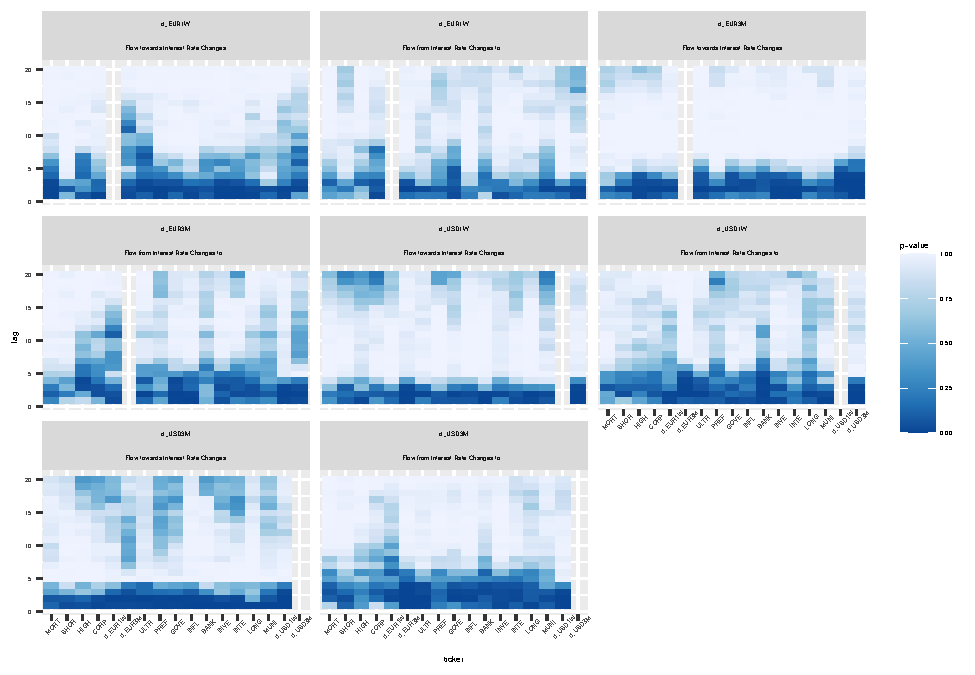
\includegraphics{working_paper_files/figure-latex/full-1.pdf}
\caption{Full period grid search results}
\end{figure}

\begin{figure}
\centering
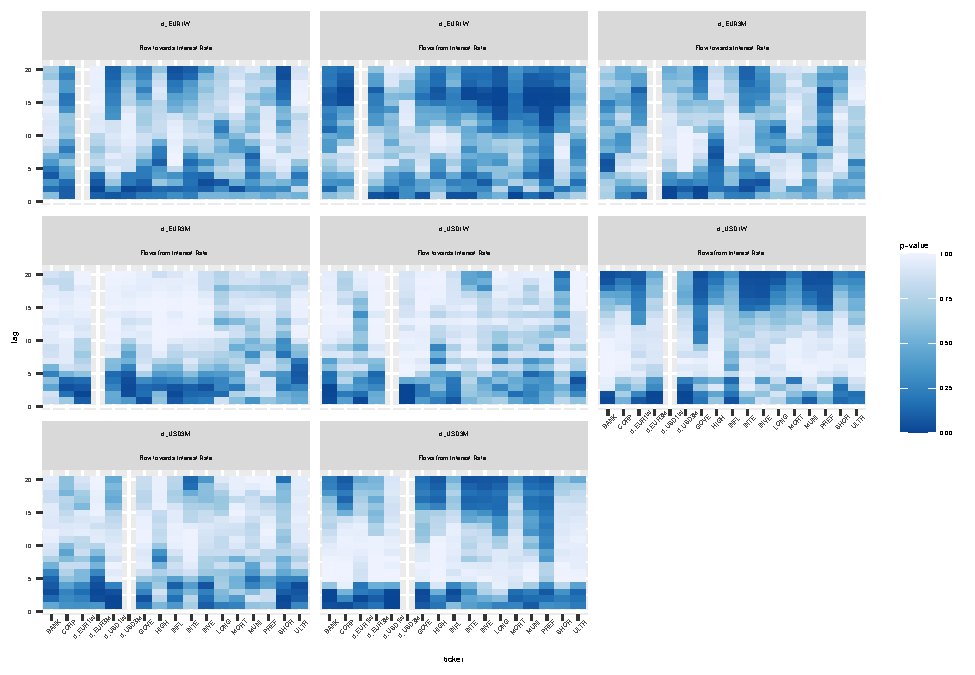
\includegraphics{working_paper_files/figure-latex/CE-1.pdf}
\caption{Credit Easing period grid search results}
\end{figure}

\begin{figure}
\centering
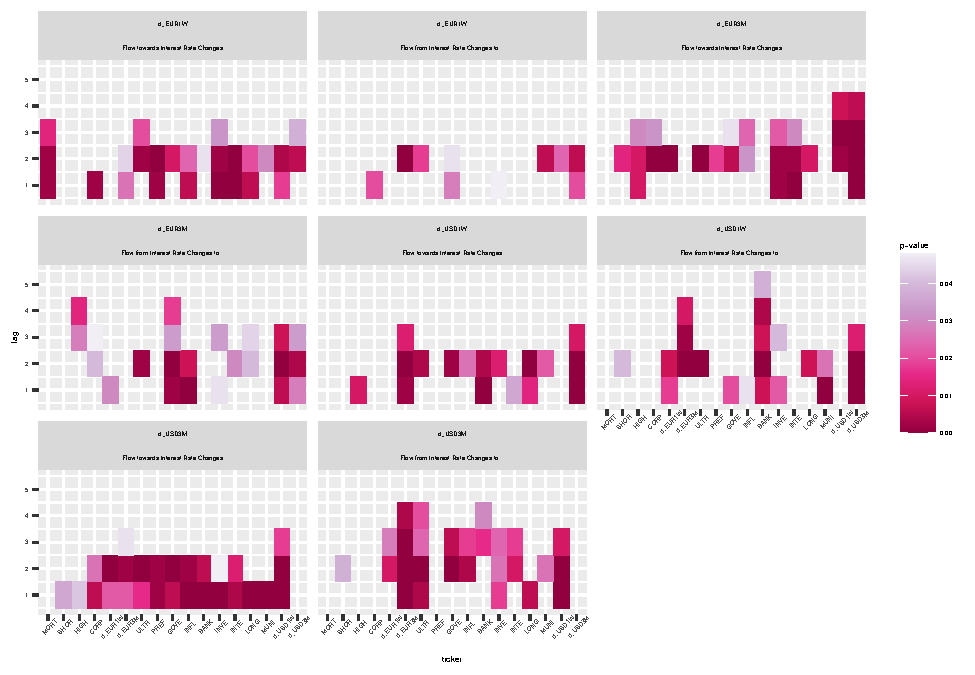
\includegraphics{working_paper_files/figure-latex/fullless5-1.pdf}
\caption{Full period grid search results (p value\textless5\%)}
\end{figure}

\begin{figure}
\centering
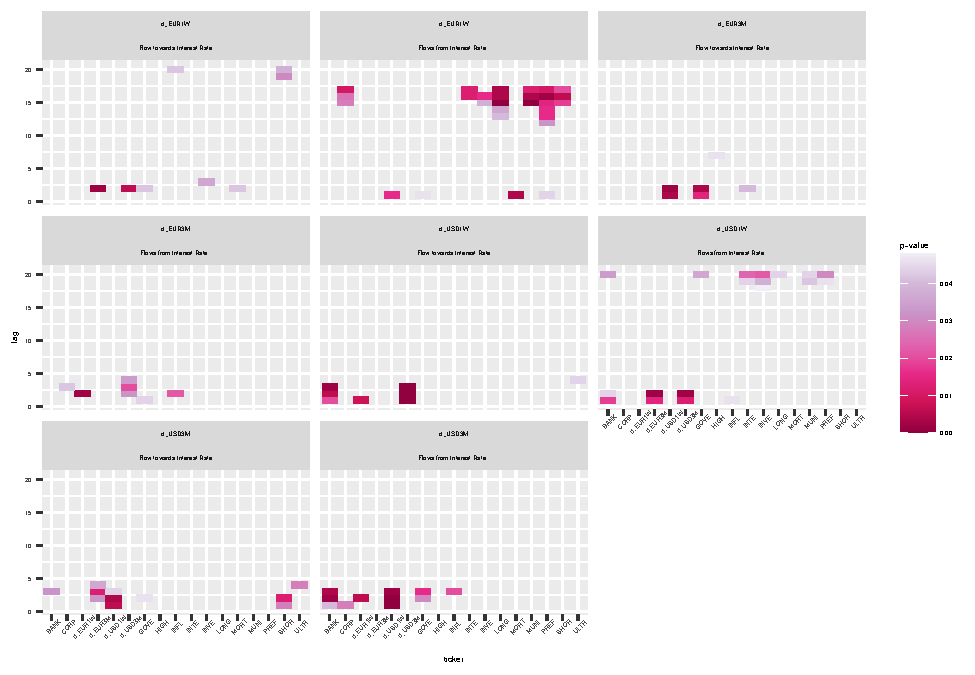
\includegraphics{working_paper_files/figure-latex/CE1-1.pdf}
\caption{Credit Easing period grid search results (p value \textless{}
5\%)}
\end{figure}

\hypertarget{false-discovery-correction}{%
\subsection{False discovery
correction}\label{false-discovery-correction}}

The previous procedure treats each effective transfer entropy estimates
as independent when considering their level of significance. As we have
over 2000 NHST p-values this is a unrealistic assumption.The replication
crisis in finance has shown that researchers routinely explicitly or
implicitly ignore multiple comparison bias and do not control for false
discovery. This has lead many to assert that most research findings use
the standard null hypothesis significance testing are likely false
(Campbell ,2017). We correct for false discovery by applying the
procedure first set in Benjamini and Hochberg (1995). Astonishingly,
this correction is little used in finance, where since its publication
this paper has bee citied over 50000 times.

\begin{figure}
\centering
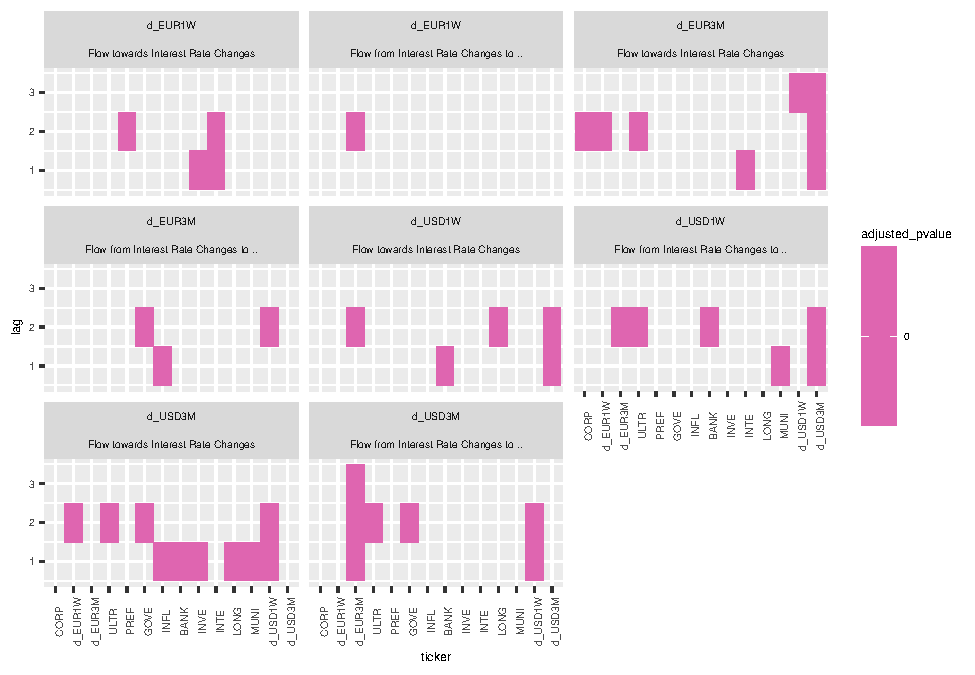
\includegraphics{working_paper_files/figure-latex/fullless6-1.pdf}
\caption{Full period grid search results (adjusted p value\textless5\%)}
\end{figure}

\begin{figure}
\centering
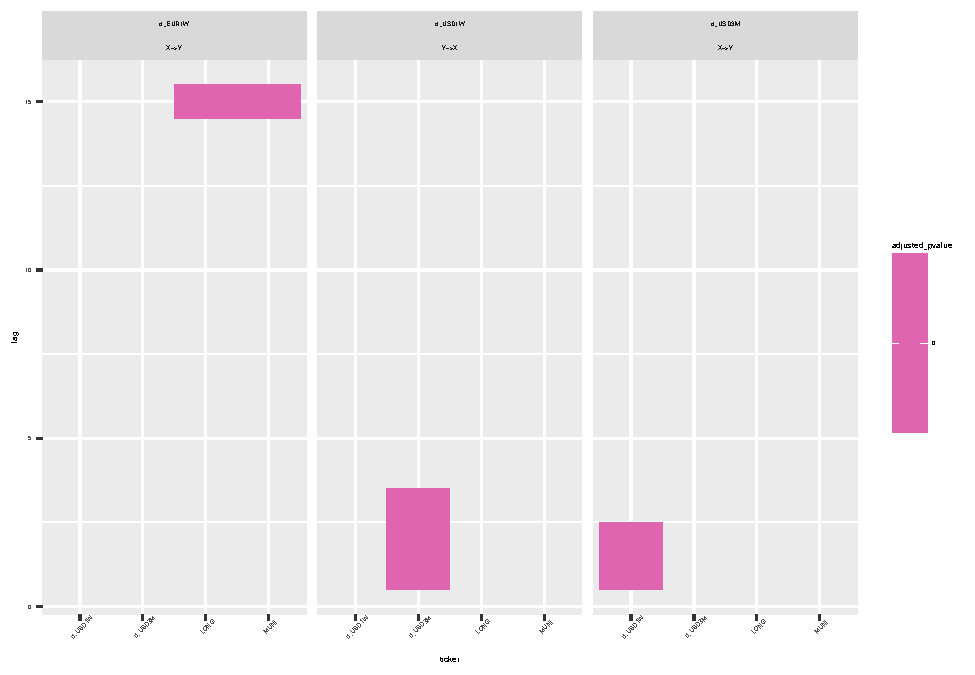
\includegraphics{working_paper_files/figure-latex/CE7-1.pdf}
\caption{Credit Easing period grid search results (adjusted p
value\textless5\%)}
\end{figure}

\hypertarget{reference}{%
\section{Reference}\label{reference}}

Benjamini, Y. \& Hochberg, Y. Controlling the False Discovery Rate: A
Practical and Powerful Approach to Multiple Testing. J Royal Statistical
Soc Ser B Methodol 57, 289--300 (1995).

R, H., Campbell. Presidential address: The scientific outlook in
finance. J Finance 72, 1399--1440 (2017).

Lundberg, S. M., \& Lee, S.-I. (2017). A unified approach to
interpreting model predictions. Proceedings of the 31st International
Conference on Neural Information Processing Systems, 4768--4777.

Brandt, P. T., Colaresi, M., \& Freeman, J. R. (2008). The Dynamics of
Reciprocity, Accountability, and Credibility. The Journal of Conflict
Resolution, 52(3), 343--374.

Brandt, P. T., \& Freeman, J. R. (2006). Advances in Bayesian Time
Series Modeling and the Study of Politics: Theory Testing, Forecasting,
and Policy Analysis. Political Analysis: An Annual Publication of the
Methodology Section of the American Political Science Association,
14(1), 1--36.

Brandt, P. T., Freeman, J. R., \& Schrodt, P. A. (2014). Evaluating
forecasts of political conflict dynamics. International Journal of
Forecasting, 30(4), 944--962.

Beck, Christian, and Friedrich Schögl. 1993. Thermodynamics of Chaotic
Systems: An Introduction. Cambridge Nonlinear Science Series 4.
Cambridge University Press.

Dimpfl, Thomas, and Franziska Julia Peter. 2013. ``Using Transfer
Entropy to Measure Information Flows Between Financial Markets.''
Studies in Nonlinear Dynamics and Econometrics 17 (1): 85--102.

Jizba, Petr, Hagen Kleinert, and Mohammad Shefaat. 2012. ``Renyi's
Information Transfer Between Financial Time Series.'' Physica A 391:
2971--89.

Kullback, S., and R. A. Leibler. 1951. ``On Information and
Sufficiency.'' The Annals of Mathematical Statistics 1: 79--86.

Marschinski, R., and H. Kantz. 2002. ``Analysing the Information Flow
Between Financial Time Series: An Improved Estimator for Transfer
Entropy.'' European Physical Journal B 30 (2): 275--81.

Shannon, C. E. 1948. ``A Mathematical Theory of Communication.'' Bell
System Technical Journal 27: 379--423.

Sims, C. A., Waggoner, D. F., \& Zha, T. (2008). Methods for inference
in large multiple-equation Markov-switching models. Journal of
Econometrics, 146(2), 255--274.

Sims, C. A., \& Zha, T. (1998). Bayesian Methods for Dynamic
Multivariate Models. International Economic Review, 39(4), 949--968.

Sims, C. A., \& Zha, T. (2006). Were There Regime Switches in U.S.
Monetary Policy? The American Economic Review, 96(1), 54--81.

Behrendt, S., Dimpfl, T., Peter, F. J., \& Zimmermann, D. J. (2019).
RTransferEntropy --- Quantifying information flow between different time
series using effective transfer entropy. SoftwareX, 10, 100265.

\end{document}
